% !TEX root = saveliev_physics_general_course_1.tex
%!TEX TS-program = pdflatex
%!TEX encoding = UTF-8 Unicode

%\chapter{THE LIQUID STATE}\label{chap:14}

\chapter{TRẠNG THÁI LỎNG}\label{chap:14}

%\section{The Structure of Liquids}\label{sec:14_1}

\section{Cấu trúc của các chất lỏng}\label{sec:14_1}

%The liquid state, occupying an intermediate position between gases and crystals, combines some features of both of these states. In particular, liquids, like crystalline substances, are characterized by having a definite volume. At the same time, a liquid, like a gas, takes on the shape of the vessel containing it. Further, the crystalline state is characterized by the ordered arrangement of the particles (atoms or molecules), whereas from this viewpoint, complete chaos reigns in gases. As shown by radiographic studies, liquids also occupy an intermediate position with respect to the nature of arrangement of their particles. The so-called \textbf{short-range order} is observed in the arrangement of liquid particles. This signifies that with respect to any particle, the arrangement of its closest neighbours is ordered. But as we move farther and farther away from a given particle, the arrangement of other particles relative to it becomes less and less ordered, and order in the arrangement of the particles vanishes quite rapidly. In crystals, there is \textbf{long-range order}: the ordered arrangement of particles with respect to any particle is observed within the limits of an appreciable volume.

Trạng thái lỏng, do ở chỗ chiếm vị trí trung gian giữa các chất khí và các tinh thể, sẽ mang một số nét của cả hai trạng thái đó. Đặc biệt đối với các chất lỏng cũng như đối với các chất kết tinh, nét đặc trưng là có một thể tích nhất định, và đồng thời chất lỏng, giống như chất khí, lấy hình dạng của bình chứa nó. Hơn nữa, đối với trạng thái kết tinh, nét đặc trưng là sự sắp xếp có trật tự của các hạt (các nguyên tử hoặc các phân tử), trong các chất khí thì sự hỗn loạn hoàn toàn thống trị. Theo những nghiên cứu ảnh chụp bằng tia Röntgen, về đặc trưng, các cách sắp xếp các hạt chất lỏng cũng chiếm một vị trí trung gian. Trong sự sắp xếp các hạt chất lỏng, người ta quan sát thấy cái gọi là \textbf{trật tự gần}. Điều đó có nghĩa là đối với bất kỳ một loại hạt nào, sự sắp xếp của các hạt lân cận gần nó nhất cũng có trật tự. Tuy nhiên, khi đi xa dần khỏi hạt đã cho sự sắp xếp các hạt hoàn toàn biến mất một cách khá nhanh chóng. Trong các tinh thể có \textbf{trật tự xa}: sự sắp xếp có trật tự của các hạt đối với bất kỳ một loại hạt nào cũng xuất hiện trong phạm vi một thể tích đáng kể.

%The presence of short-range order in liquids is the reason why their structure is called \textbf{quasicrystalline} (crystal-like).

Sự có mặt của tính trật tự gần trong các chất lỏng là nguyên nhân tại sao người ta thường gọi cấu trúc của chất lỏng là cấu trúc \textbf{giả kết tinh} (cấu trúc tựa tinh thể).

%Owing to the absence of long-range order in them, liquids, with a few exceptions, do not display the anisotropy characteristic of crystals with their regular arrangement of the particles. Liquids with elongated molecules display an identical orientation of their molecules within a considerable volume, which results in anisotropy of their optical and some other properties. Such liquids are known as liquid crystals. Only the orientation of the molecules is ordered in them, while the mutual arrangement of the molecules, as in conventional liquids, does not display long-range order.

Do ở chỗ không có tính trật tự xa nên người ta không phát hiện thấy tính dị hướng của các chất lỏng, trừ một số ít trường hợp ngoại lệ; tính dị hướng là một tính chất đặc thù của các tinh thể có sự sắp xếp đều đặn của các hạt. Trong những chất lỏng có các phân tử kéo dài người ta quan sát thấy có sự định hướng như nhau của các phân tử trong phạm vi một thể tích tương đối lớn, đó là nguyên nhân của sự dị hướng của các tính chất quang học cũng như của một số tính chất khác. Các chất lỏng đó gọi là các \textbf{tinh thể lỏng}. Ở các tinh thể lỏng, chỉ có sự định hướng của các phân tử là có trật tự, sự sắp xếp tương hỗ của các phân tử như trong các chất lỏng thông thường, người ta không phát hiện ra tính trật tự xa.

%The circumstance that the liquid state is especially complicated as regards its properties is due to the intermediate position of liquids. Therefore, its theory has been developed to a much smaller extent than that of the crystalline and gaseous states. To date there is no complete and universally recognized theory of liquids. Considerable merit in developing a number of problems of the theory of the liquid state belongs to the Soviet scientist Yakov Frenkel (1894-1952).

Do ở chỗ các chất lỏng chiếm một vị trí trung gian nên trạng thái lỏng có những tính chất đặc biệt phức tạp. Vì vậy lý thuyết về trạng thái lỏng rất kém phát triển so với các lý thuyết về trạng thái kết tinh và trạng thái khí. Cho đến nay chưa có lý thuyết về chất lỏng hoàn toàn đầy đủ và được mọi người thừa nhận. Nhà bác học Soviet Yakov Frenkel (1894-1952) có công lao đáng kể trong việc phát triển một loại vấn đề về lý thuyết của trạng thái lỏng.

%Frenkel postulates that the thermal motion in liquids has the following nature. Each molecule during a certain time oscillates about a definite position of equilibrium. The molecule changes its place of equilibrium from time to time, moving in a jump to a new position that is at a distance from the previous one of the order of the size of the molecules themselves. The molecules thus move only slowly inside a liquid, spending part of their time near definite places. As picturesquely expressed by Frenkel, the molecules wander throughout the entire volume of a liquid, leading a nomadic mode of life in which brief removals are replaced by relatively long periods of settled life. The lengths of these stops vary quite considerably and chaotically alternate with one another, but the mean duration of oscillations about a single equilibrium position is a definite quantity. for each liquid that sharply diminishes with increasing temperature. In this connection, elevation of the temperature is attended by a great growth in the mobility of the molecules, and this, in turn, results in diminishing of the viscosity of the liquid.

Theo Frenkel, chuyển động nhiệt trong các chất lỏng có tính chất sau đây. Trong một khoảng thời gian nào đó, mỗi phân tử dao động quanh một vị trí cân bằng xác định. Thỉnh thoảng phân tử thay đổi vị trí cân bằng của nó bằng một cái nhảy cóc sang một vị trí cân bằng mới nằm cách vị trí cân bằng cũ một khoảng cách vào cỡ kích thước của chính các phân tử. Vì vậy, các phân tử chỉ dịch chuyển chậm trong chất lỏng, sống một phần thời gian quanh những vị trí xác định. Theo sự diễn tả có tính chất hình tượng của Frenkel, các phân tử chu du trong toàn bộ thể tích chất lỏng, sống một cuộc sống du mục trong đó có những cuộc di chuyển ngắn xen kẽ với những thời kỳ sống định cư tương đối dài. Độ dài của những thời gian dừng lại đó rất khác nhau và thay đổi một cách hỗn loạn, nhưng độ dài trung bình của thời gian dao động quanh vị trí cân bằng là một đại lượng xác định đối với mỗi chất lỏng; thời gian này giảm rất nhanh khi tăng nhiệt độ. Do đó, khi tăng nhiệt độ thì độ linh động của các phân tử tăng rất mạnh, điều đó lại dẫn đến hệ quả là làm giảm độ nhớt của chất lỏng.

%Solids exist that in many respects are closer to liquids than to crystals. Such substances, called \textbf{amorphous}, do not display anisotropy. Only short-range order is encountered in the arrangement of their particles. The transition from an amorphous solid to a liquid when such a substance is heated occurs continuously, whereas the transition from a crystal to a liquid occurs in a jump (this will be treated in greater detail in Sec.~\ref{sec:15_6}). All this gives us grounds to consider amorphous solid substances as supercooled liquids whose particles owing to the greatly increased viscosity have a limited mobility.

Có những chất rắn về nhiều phương diện tỏ ra gần các chất lỏng hơn là các tinh thể. Các chất đó là các \textbf{chất vô định hình}, chúng không có tính dị hướng. Cũng như ở các chất lỏng, trong sự sắp xếp các hạt của chúng chỉ có sự trật tự gần. Sự chuyển từ các chất rắn vô định hình sang các chất lỏng khi đun nóng được thực hiện một cách liên tục, trong khi đó thì sự chuyển từ một tinh thể sang chất lỏng được thực hiện bằng một bước nhảy (ta sẽ trình bày chi tiết hơn về vấn đề này trong mục.~\ref{sec:15_6}). Tất cả điều đó cho ta cơ sở để coi các chất rắn vô định hình như các chất lỏng đông lạnh; do ở độ nhớt tăng rất mạnh nên các hạt của chúng có độ linh động rất nhỏ. 

%A typical example of an amorphous solid is glass. Amorphous substances also include resins and bitumens.

Thuỷ tinh là một thí dụ điển hình về chất rắn vô định hình. Trong số các chất vô định hình còn có hắc ín, nhựa đường v.v...

%\section{Surface Tension}\label{sec:14_2}

\section{Sức căng mặt ngoài}\label{sec:14_2}

%The molecules of a liquid are so close to one another that the forces of attraction between them have a considerable value. Since the interaction rapidly falls off with the distance, beginning from a certain distance the forces of attraction between the molecules may be disregarded. This distance $r$, as we already know (see Sec.~\ref{sec:10_13}), is called the \textbf{radius of molecular action}, and a sphere of radius $r$ is called a \textbf{sphere of molecular action}. The radius of molecular action has a magnitude of the order of several effective diameters of a molecule.

Các phân tử chất lỏng ở gần nhau đến nỗi các lực hút giữa chúng có độ lớn đáng kể. Vì sự tương tác giảm rất nhanh theo khoảng cách, nên bắt đầu từ một khoảng cách nào đó, có thể bỏ qua các lực hút giữa các phân tử. Như chúng ta đã biết, khoảng cách $r$ đó gọi là \textbf{bán kính tác dụng phân tử} (xem Mục.~\ref{sec:10_13}), còn hình cầu bán kính $r$ gọi là \textbf{hình cầu tác dụng phân tử}. Bán kính tác dụng phân tử có độ lớn vào cỡ một vài đường kính hiệu dụng của phân tử.

%Each molecule is attracted by all its neighbour molecules within the limits of the sphere of molecular action whose centre coincides with the given molecule. The resultant of all these forces for a molecule that is at a distance from the surface of the liquid exceeding $r$ evidently equals zero on the average (\fig{14_1}). Matters are different if a molecule is at a distance less than $r$ from the surface. Since the density of the vapour (or gas with which the liquid has an interface) is much smaller than that of the liquid, the part of the sphere of molecular action protruding beyond the limits of the liquid will be filled with fewer molecules than the remaining part of the sphere. As a result, every molecule in a surface layer of thickness $r$ will experience a force directed into the liquid. The magnitude of this force grows in a direction from the inner to the outer boundary of the layer.

Mỗi phân tử chịu lực hút của tất cả các phân tử ở cạnh nó nằm trong phạm vi của một hình cầu tác dụng phân tử có tâm trùng với phân tử đã cho. Đối với phân tử nằm các bề mặt của chất lỏng một khoảng lớn hơn $r$ thì tổng hợp của tất cả các lực tác dụng lên nó dĩ nhiên về trung bình là bằng không (\fig{14_1}). Nếu phân tử nằm cách bề mặt chất lỏng một khoảng nhỏ hơn $r$ thì vấn đề sẽ khác. Vì mật độ của hơi (hoặc khí giới hạn chất lỏng) nhỏ hơn mật độ của chất lỏng nhiều lần, nên phần của hình cầu tác dụng phân tử ló ra ngoài giới hạn của chất lỏng sẽ chứa ít phân tử hơn phần còn lại của hình cầu. Kết quả là trên mỗi phân tử nằm ở trong lớp bề mặt có độ dày $r$ sẽ có một lực tác dụng hướng vào phía bên trong chất lỏng. Cường độ của lực đó tăng theo hướng đi từ bờ bên trong của lớp đó ra bờ bên ngoài.

\begin{figure}[!htb]
	\begin{center}
		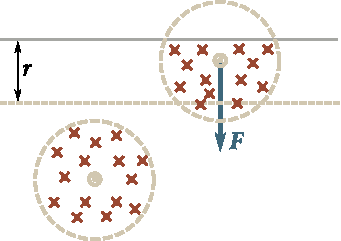
\includegraphics[scale=1.1]{figures/ch_14/fig_14_1.pdf}
		\caption[]{}
		\label{fig:14_1}
	\end{center}
	\vspace{-0.8cm}
\end{figure}

%The transition of a molecule from the bulk of a liquid to its surface layer is associated with the need to do work against the forces acting in the surface layer. This work is done by the molecule at the expense of its store of kinetic energy and increases the potential energy of the molecule, just as the work done by a body flying upward against the forces of the Earth's attraction increases the potential energy of the body. When the molecule returns in to the bulk of the liquid, the potential energy which the molecule had in the surface layer transforms into the kinetic energy of the molecule.

Sự chuyển một phân tử từ trong lòng chất lỏng ra lớp mặt ngoài gắn liền với sự cần thiết phải thực hiện một công chống những lực tác dụng ở lớp mặt ngoài. Nhờ lấy ở dự trữ động năng mà phân tử thực hiện được công đó, và công này làm tăng thế năng của phân tử; điều này giống như một vật bay lên cao đã thực hiện một công chống lại lực hấp dẫn của Trái đất, công này làm tăng thế năng của vật. Trong sự chuyển ngược lại của phân tử vào trong lòng chất lỏng, thế năng mà phân tử có được ở trong lớp mặt ngoài sẽ biến thành động năng của phân tử.

%Thus, molecules in a surface layer have an additional potential energy. The surface layer as a whole has an additional energy forming part of the internal energy of the liquid. 

Như vậy các phân tử ở trong lớp mặt ngoài có một thế năng phụ. Toàn bộ lớp mặt ngoài có một năng lượng phụ; năng lượng này là một phần cấu thành nội năng của chất lỏng.

%Since the equilibrium position corresponds to a minimum of potential energy, a liquid left to itself will take on a shape having the minimum surface area, \ie, the shape of a sphere. What we usually observe are not liquids ``left to themselves'', but liquids subjected to the action of the Earth's gravitational forces. In this case, the liquid takes on a shape corresponding to a minimum of the total energy---that in the field of the gravitational forces and the surface energy.

Vì rằng vị trí cân bằng ứng với cực tiểu của thế năng nên chất lỏng sẽ tự lấy hình dạng có bề mặt nhỏ nhất, tức là dạng hình cầu. Thông thường ta không quan sát được những chất lỏng ``tự thể hiện'' mà là những chất lỏng chịu tác dụng của các lực hấp dẫn của Trái đất. Trong trường hợp đó chất lỏng sẽ có dạng ứng với cực tiểu của năng lượng toàn phần---năng lượng trong trường lực hấp dẫn và năng lượng mặt ngoài.

%When the dimensions of a body increase, its volume grows as the cube of the linear dimensions, and its surface area only as the square of these dimensions. Therefore, the energy in the gravitational field proportional to the volume of a body changes more rapidly with increasing dimensions of the body than its surface energy. In small drops of a liquid, the surface energy plays the predominate part, and as a result the drops have a shape close to a spherical one. Large drops of a liquid flatten under the action of gravitational forces notwithstanding the fact that their surface energy grows. Large bodies of a liquid take on the shape of the vessel containing them and a horizontal free surface.

Khi tăng các kích thước của vật thì thể tích tăng theo lập phương của kích thước dài, còn bề mặt chỉ tăng theo bình phương của kích thước dài. Vì vậy, năng lượng của vật trong trường hấp dẫn, do ở chỗ tỷ lệ với thể tích của vật, sẽ thay đổi theo kích thước nhanh hơn là năng lượng mặt ngoài. Ở những giọt chất lỏng nhỏ năng lượng mặt ngoài chiếm ưu thế, do đó những giọt này có dạng gần với hình cầu. Những giọt chất lỏng lớn bị bẹt ra dưới tác dụng của các lực hấp dẫn, mặc dù năng lượng mặt ngoài khi đó tăng lên. Những khối lớn chất lỏng sẽ có hình dạng của bình chứa chúng với mặt thoáng nằm ngang. 

%The presence of surface energy causes a liquid to tend to reduce its surface area. The liquid behaves as if it were confined inside an elastic stretched out film tending to compress. It must be borne in mind that there is actually no film confining a liquid from the outside. The surface layer consists of the same molecules as the bulk of the liquid, and the interaction between the molecules in the surface layer is of the same nature as in the interior. The matter is only that the molecules in the surface layer have an additional energy in comparison with those in the bulk of the liquid.

Do sự có mặt của năng lượng mặt ngoài nên ta thấy chất lỏng có xu hướng co hẹp mặt ngoài của nó. Chất lỏng xử sự dường như nó bị nhốt trong một cái màng căng đàn hồi, màng này có xu hướng co lại. Cần phải thấy rằng thực ra không có một cái màng nào hết giới hạn bên ngoài chất lỏng. Lớp mặt ngoài cũng cấu tạo bởi những phân tử như là các phân tử của toàn bộ chất lỏng, và tương tác giữa các phân tử ở lớp mặt ngoài có cùng đặc tính như tương tác giữa các phân tử trong chất lỏng. Vấn đề là ở chỗ các phân tử ở lớp mặt ngoài có một năng lượng bổ sung so với các phân tử ở bên trong chất lỏng.

%Let us mentally separate a part of the surface of a liquid confined within a closed contour. The tendency of this portion to contract results in that it acts on the portions bordering on it with forces distributed over the entire contour (according to Newton's third law, the external portions of the surface layer act on the portion of the surface being considered with forces of the same magnitude, but opposite in direction). These forces are called forces of \textbf{surface tension}. The force of surface tension is directed along a tangent to the surface of the liquid perpendicularly to the portion of the contour it is acting upon.

Ta cắt tưởng tượng một phần mặt ngoài của chất lỏng được giới hạn vởi một chu tuyến đóng. Xu hướng co hẹp lại của phần mặt ngoài đó dẫn tới việc là nó tác dụng lên những phần tiếp giáp với nó những lực phân bố dọc theo toàn bộ chu tuyến (theo định luật Newton thứ ba những phần bên ngoài của lớp mặt ngoài tác dụng lên phần mặt ngoài đang xét với những lực có cùng cường độ, nhưng có hướng ngược lại). Những lực này gọi là các \textbf{lực căng mặt ngoài}. Lực căng mặt ngoài theo tiếp tuyến với mặt ngoài chất lỏng và vuông góc với phần chu tuyến mà nó tác dụng.

%Let us denote the force of surface tension per unit of length of a contour by $\sigma$. This quantity is defined as the surface tension. It is measured in newtons per metre (in the SI system) or in dynes per centimetre (in the cgs system).

Ta ký hiệu lực căng mặt ngoài tác dụng lên một đơn vị độ dài của chu tuyến là $\sigma$. Người ta gọi đại lượng này là suất căng mặt ngoài. Suất căng mặt ngoài được đo bằng đơn vị newton metre (trong hệ SI) hoặc dyne centimetre (trong hệ CGS).

\begin{figure}[!htb]
	\begin{center}
		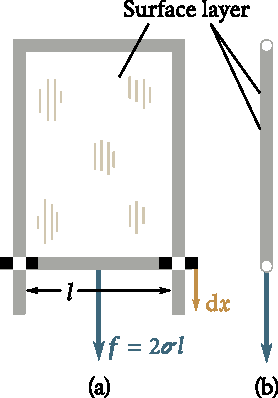
\includegraphics[scale=1.1]{figures/ch_14/fig_14_2.pdf}
		\caption[]{}
		\label{fig:14_2}
	\end{center}
	\vspace{-0.8cm}
\end{figure}

%Assume that we have a rectangular frame with a movable side confining a film of a liquid (\fig{14_2}). A film is a thin flat volume of liquid confined on both sides by a surface layer (see \fig{14_2}b in which a cross section of the frame is shown). Owing to the tendency of the surface layer to contract, the film will exert a force equal to $2\sigma l$ on the movable side. For the latter to be in equilibrium, an external force $f$ must be applied to it that equals the force tensioning the film, \ie, $2\sigma l$. Let us assume that the movable side has moved very slowly in the direction of action of the force $f$ over the very small distance $\deriv{x}$. This process is attended by the liquid above the movable side doing the work $\derivp{A}=-2\sigma l\,\deriv{x}=-\sigma\,\deriv{S}$, where $\deriv{S}$ is the increment of the area of the surface layer. With such an increase of the surface, an additional number of molecules will pass from the interior of the liquid to the surface layer, losing their velocity. Therefore, if the process proceeded adiabatically, the liquid would cool slightly. We assumed, however, that the process goes on very slowly (reversibly), owing to which the temperature of the film remains constant as a result of the inflow of heat from the surroundings. Thus, the process will go on isothermally.

Giả sử ta có một khung hình chữ nhật có một xà ngang di chuyển được và một màng chất lỏng căng trên khung đó (\fig{14_2}). Màng này chính là một khối chất lỏng phẳng, mỏng, giới hạn bởi hai lớp mặt ngoài ở hai bên (xem \fig{14_2}b, trên hình đó ta vẽ mặt cắt của khung). Do ở xu hướng co ngắn của lớp mặt ngoài, màng sẽ tác dụng lên xà ngang một lực bằng $2\sigma l$. Muốn cho xà ngang nằm ngang cân bằng, ta phải tác dụng lên nó một ngoại lực $f$ bằng lực căng mặt ngoài của màng, tức là bằng $2\sigma l$. Giả sử xà ngang di chuyển rất chậm theo hướng tác dụng của lực $f$ một đoạn đường rẩt nhỏ $\deriv{x}$. Quá trình đó kèm theo sự thực hiện công $\derivp{A}=-2\sigma l\,\deriv{x}=-\sigma\,\deriv{S}$ của chất lỏng tác dụng lên xà ngang, trong đó $\deriv{S}$ là độ tăng diện tích lớp mặt ngoài. Khi mặt ngoài tăng lên như vậy có một số phân tử bổ sung chuyển từ trong lòng chất lỏng ra lớp mặt ngoài, đồng thời mất đi vận tốc của mình. Vì vậy, nếu quá trình diễn ra một cách đoạn nhiệt thì chất lỏng sẽ hơi lạnh đi một chút. Tuy nhiên ta đã giả thiết là quá trình xảy ra rất chậm (thuận nghịch), do đó nhiệt độ của màng vẫn không đổi do nó lấy nhiệt từ bên ngoài. Vì vậy quá trình sẽ xảy ra một cách đẳng nhiệt.

%We established in Sec.~\ref{sec:12_6} that the work done in a reversible isothermal process equals the decrement of the free energy [see \eqn{12_56}]. We can therefore write that

Trong Mục.~\ref{sec:12_6} ta đã thấy là công được thực hiện trong một quá trình đẳng nhiệt thuận nghịch sẽ bằng độ giảm năng lượng tự do [xem \eqn{12_56}]. Do đó, có thể viết là

\begin{equation*}
	\derivp{A} = -\sigma\,\deriv{S} = -\deriv{F}.
\end{equation*}

\noindent

%The result obtained signifies that upon an isothermal increase in the area of the surface layer by $\deriv{S}$, the free energy of the liquid grows by $\deriv{F}=\sigma\,\deriv{S}$. It thus follows that the surface tension $\sigma$ is the additional free energy which a unit area of a surface layer has. Accordingly, $\sigma$ can be expressed not only in newtons per metre (or dynes per centimetre), but also in joules per square metre (or in ergs per square centimetre).

Kết quả thu được có nghĩa là khi tăng đẳng nhiệt diện tích lớp mặt ngoài lên một lượng $\deriv{S}$ thì năng lượng tự do của chất lỏng sẽ tăng một lượng là $\deriv{F}=\sigma\,\deriv{S}$. Từ đó suy ra rằng suất căng mặt ngoài $\sigma$ chính là phần năng lượng tự do bổ sung của một đơn vị diện tích lớp mặt ngoài. Vì vậy, có thể biểu thị $\sigma$ không những bằng newtons trên metre (hoặc dynes trên centimetre) mà còn bằng joules trên metre vuông (hoặc ergs trên centimetre vuông).

%Impurities greatly affect the magnitude of the surface tension. For example, soap dissolved in water reduces its surface tension almost one-and-a-half times. When \ce{NaCl} is dissolved in water, on the contrary, the surface tension grows.

Các tạp chất ảnh hưởng rất mạnh đến độ lớn của sức căng mặt ngoài. Chẳng hạn khi hoà tan xà phòng vào nước, suất căng mặt ngoài của nước sẽ giảm đi một lần rưỡi. Khi hoà tan \ce{NaCl} vào nước, trái lại, $\sigma$ sẽ tăng lên.

%With elevation of the temperature, the difference between the densities of a liquid and its saturated vapour diminishes (see Sec.~\ref{sec:15_4}). In this connection, the surface tension also decreases. At the critical temperature (its definition is given in Sec.~\ref{sec:15_4}), $\sigma$ vanishes.

Khi tăng nhiệt độ, sự khác nhau giữa mật độ của chất lỏng và của hơi bão hoà của nó sẽ giảm bớt (xem Phần.~\ref{sec:15_4}). Do đó suất căng mặt ngoài cũng giảm. Ở nhiệt độ tới hạn (trong Phần.~\ref{sec:15_4} sẽ cho định nghĩa về nhiệt độ tới hạn), $\sigma$ sẽ bằng không.

%\section{Pressure under a Curved Liquid Surface}\label{sec:14_3}

\section{Áp suất dưới mặt cong của chất lỏng}\label{sec:14_3}

%Let us consider the surface of a liquid resting on a flat contour (\fig{14_3}a). If the surface of the liquid is not flat, its tendency to decrease its area leads to the appearance of a pressure apart from that exerted on a liquid with a flat surface. When the surface is convex, this additional pressure is positive (\fig{14_3}b), and when it is concave, this pressure is negative (\fig{14_3}c). In the last case, the surface layer, tending to diminish, stretches the liquid.

Ta hãy xét một mặt chất lỏng tựa trên một chu tuyến phẳng nào đó (\fig{14_3}a). Nếu mặt chất lỏng phẳng thì xu hướng co bề mặt chất lỏng sẽ dẫn tới sự xuất hiện một áp suất phụ bổ sung vào áp suất tác dụng chất lỏng khi mặt ngoài phẳng. Trong trường hợp mặt ngoài lồi thì áp suất phụ đó sẽ dương (\fig{14_3}b), trong trường hợp mà mặt ngoài lõm thì áp suất phụ sẽ âm (\fig{14_3}c). Trong trường hợp sau, khi lớp mặt ngoài cố co lại, nó sẽ kéo dãn chất lỏng ra.

\begin{figure}[!htb]
	\begin{center}
		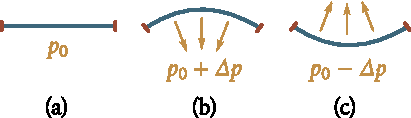
\includegraphics[scale=1.1]{figures/ch_14/fig_14_3.pdf}
		\caption[]{}
		\label{fig:14_3}
	\end{center}
	\vspace{-0.8cm}
\end{figure}

%The magnitude of the additional pressure must obviously grow with an increasing surface tension $\sigma$ and surface curvature. Let us calculate the additional pressure for a spherical surface of a liquid. To do this, we shall mentally cut a spherical drop of a liquid with a diametral plane into two hemispheres (\fig{14_4}). Owing to surface tension, both hemispheres are attracted to each other with a force equal to

Độ lớn của áp suất phụ dĩ nhiên phải tăng khi tăng suất căng mặt ngoài $\sigma$ và độ cong của mặt. Ta tính áp suất phụ đối với mặt ngoài chất lỏng hình cầu. Muốn vậy ta hãy tưởng tượng cắt giọt chất lỏng hình cầu thành hai bán cầu bằng một mặt phẳng xuyên tâm (\fig{14_4}). Do sức căng mặt ngoài nên cả hai bán cầu hút lẫn nhau với một lực bằng

\begin{equation*}
	f = l\sigma = 2\pi R\sigma.
\end{equation*}

\noindent

%This force presses the two hemispheres against each other over the surface $S=\pi R^2$ and, consequently, produces the additional pressure
Lực đó ép cả hai bán cầu vào nhau theo bề mặt $S=\pi R^2$, và do đó gây ra áp suất phụ

\begin{equation}\label{eq:14_1}
	\Delta p = \frac{f}{S} = \frac{2\pi R\sigma}{\pi R^2} = \frac{2\sigma}{R}.
\end{equation}

%The curvature of a spherical surface is the same everywhere and is determined by the radius of the sphere $R$. It is obvious that the smaller the radius $R$, the greater is the curvature of a spherical surface. It is customary practice to characterize the curvature of an arbitrary surface by the so-called mean curvature, which may differ for various points of a surface.

Độ cong của mặt cầu là như nhau ở mọi chỗ và được xác định bằng bán kính $R$ của hình cầu. Rõ ràng là khi $R$ càng nhỏ thì độ cong của mặt cầu lại càng lớn. Độ cong của một mặt bất kỳ thường được đặc trưng bằng độ cong trung bình; đại lượng này có thể khác nhau ở những điểm khác nhau của bề mặt.

%The mean curvature is determined through the curvature of normal sections. A normal section of a surface at a certain point is defined as the line of intersection of this surface with a plane passing through a normal to the surface at the point being considered. For a sphere, any normal section is a circle of radius $R$ (here $R$ is the radius of the sphere). The quantity $H=1/R$ gives the curvature of a sphere. In the general case, different normal sections passing through the same point have different curvatures. It is proved in geometry that the half-sum of the reciprocal radii of curvature

Độ cong trung bình được xác định qua độ cong của các tiết diện thằng góc. Tiết diện thẳng góc của một mặt tại một điểm nào đó là giao tuyến của mặt đó với mặt phẳng đi qua pháp tuyến của mặt ở điểm mà ta xét. Đối với mặt cầu thì bất kỳ một tiết diện thằng góc nào cũng là một đường tròn bán kính $R$ ($R$ là bán kính của mặt cầu). Đại lượng $H=1/R$ là độ cong của mặt cầu. Trong trường hợp tổng quát những tiết diện thẳng góc khác nhau đi qua cùng một điểm sẽ có những độ cong khác nhau. Trong hình học người ta đã chứng minh rằng nửa tổng của các nghịch đảo của các bán kính cong các cặp tiết diện thẳng góc bất kỳ, vuông góc với nhau, sẽ có cùng một trị số:

\begin{equation}\label{eq:14_2}
	H = \frac{1}{2}\parenthesis{\frac{1}{R_1} + \frac{1}{R_2}}
\end{equation}

\noindent

%for any pair of mutually perpendicular normal sections has the same value. It is exactly this quantity that is the mean curvature of a surface at a given point.

Đại lượng đó là độ cong trung bình của mặt ở điểm đã cho. 

%The radii $R_1$ and $R_2$ in \eqn{14_2} are algebraic quantities. If the centre of curvature of a normal section is under a given surface, the relevant radius of curvature is positive; if the centre of curvature is above the surface, the radius of curvature is negative (\fig{14_5}). Thus, a curved surface can have a mean curvature equal to zero. For this purpose, the radii of curvature $R_1$ and $R_2$ must be identical in magnitude and opposite in sign.

Các bán kính $R_1$ và $R_2$ trong \eqn{14_2} là những đại lượng đại số. Nếu tâm cong của tiết diện thẳng góc nằm dưới mặt đã cho thì bán kính cong tương ứng sẽ dương; nếu tâm cong nằm trên mặt đã cho thì bán kính cong sẽ âm (\fig{14_5}). Vì vậy, một mặt không phẳng có độ cong trung bình bằng không. Muốn vậy, cần phải sao cho các bán kính cong $R_1$ và $R_2$ có độ lớn như nhau và có dấu ngược nhau.

\begin{figure}[!htb]
	\begin{minipage}[t]{0.5\linewidth}
		\begin{center}
			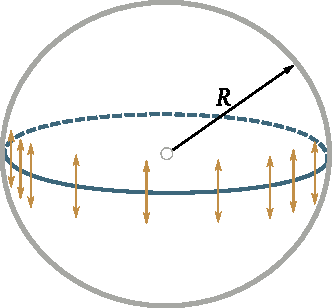
\includegraphics[scale=1]{figures/ch_14/fig_14_4.pdf}
			\caption[]{}
			\label{fig:14_4}
		\end{center}
	\end{minipage}
	\hspace{-0.05cm}
	\begin{minipage}[t]{0.5\linewidth}
		\begin{center}
			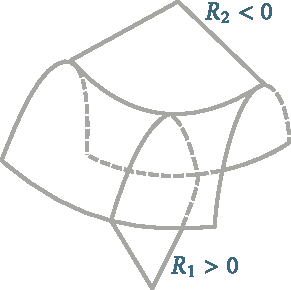
\includegraphics[scale=1]{figures/ch_14/fig_14_5.pdf}
			\caption[]{}
			\label{fig:14_5}
		\end{center}
	\end{minipage}
	\vspace{-0.4cm}
\end{figure}

%For a sphere, we have $R_1=R_2=R$, so that by \eqn{14_2}, $H=1/R$. Substituting $H$ for $1/R$ in \eqn{14_1}, we get

Đối với mặt cầu $R_1=R_2=R$, do đó theo \eqn{14_2}, $H=1/R$. Thay $1/R$ bằng $H$ trong \eqn{14_1}, ta được

\begin{equation}\label{eq:14_3}
	\Delta p = 2H\sigma.
\end{equation}
%The French scientist Pierre Laplace (1749-1827) proved that \eqn{14_3} holds for a surface of any shape if by $H$ we understand the mean curvature of a surface at the point under which the additional pressure is being determined. Introducing the expression~\eqref{eq:14_2} for the mean curvature into \eqn{14_3}, we get a formula for the additional pressure under an arbitrary surface:

Nhà khoa học người Pháp Pierre Laplace (1749-1827) đã chứng minh rằng \eqn{14_3} vẫn dùng đối với mặt có dạng bất kỳ nếu ta hiểu $H$ là độ cong trung bình của mặt ở điểm mà dưới đó ta xác định được áp suất phụ. Thế biểu thức~\eqref{eq:14_2} về độ cong trung bình vào \eqn{14_3}, ta thu được công thức tính áp suất phụ dưới mặt cong bất kỳ:
\begin{equation}\label{eq:14_4}
	\Delta p = \sigma\parenthesis{\frac{1}{R_1} + \frac{1}{R_2}}.
\end{equation}

\noindent
%It is called the \textbf{Laplace formula}.

Công thức này gọi là \textbf{công thức Laplace}.

%The additional pressure given by \eqn{14_4} causes the level of a liquid in a narrow tube (capillary) to change. This is why it is sometimes called the \textbf{capillary pressure}.

Áp suất phụ \eqn{14_4} gây ra sự thay đổi mức chất lỏng trong những ống hẹp (các ống mao dẫn), vì vậy đôi khi người ta còn gọi áp suất phụ là \textbf{áp suất mao dẫn}.

%\section{Phenomena on Liquid-Solid Interface}\label{sec:14_4}

\section{Các hiện tượng tại biên của chất lỏng và chất rắn}\label{sec:14_4}

%Everything said in Sec.~\ref{sec:14_2} about the special conditions in which the molecules of a surface layer are also relates completely to solids. Hence, solids, like liquids, have a surface tension.
Tất cả những điều trình bày trong~\ref{sec:14_2} về những điều kiện đặc biệt mà các phân tử trong lớp mặt ngoài phải chịu cũng hoàn toàn ứng với các chất rắn. Do đó, các chất rắn, cũng như các chất lỏng, đều có sức căng mặt ngoài.

%When considering phenomena on the interface between various media, we must not forget that the surface energy of a liquid or solid depends not only on the properties of the given liquid or solid, but also on the properties of the substance with which they have a common boundary. Strictly speaking, we must consider the total surface energy $\sigma_{12}$ of both substances in contact with each other (\fig{14_6}). Only if one of the substances is gaseous, does not react chemically with the other substance, and has a poor solubility in it, can we simply speak of the surface energy (or the surface tension) of the second liquid or solid.

Khi xét các hiện tượng tại biên ngăn cách những môi trường khác nhau, cần phải chú ý là năng lượng mặt ngoài của một chất lỏng hay chất rắn không những phụ thuộc vào các tính chất của chất lỏng hay chất rắn đã cho mà còn phụ thuộc vào tính chất của chất giới hạn chúng. Nói một cách chặt chẽ, cần phải xét tổng năng lượng mặt ngoài $\sigma_{12}$ của cả hai chất giới hạn lẫn nhau (\fig{14_6}). Chỉ khi một chất là chất khí không có tác dụng hoá học với chất kia và ít hoà tan vào nó, thì ta mới có thể nói đơn thuần về năng lượng mặt ngoài (hoặc suất căng mặt ngoài) của chất lỏng hay chất rắn kia.

\begin{figure}[!htb]
	\begin{minipage}[t]{0.5\linewidth}
		\begin{center}
			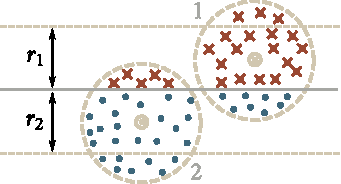
\includegraphics[scale=1]{figures/ch_14/fig_14_6.pdf}
			\caption[]{}
			\label{fig:14_6}
		\end{center}
	\end{minipage}
	\hspace{-0.05cm}
	\begin{minipage}[t]{0.5\linewidth}
		\begin{center}
			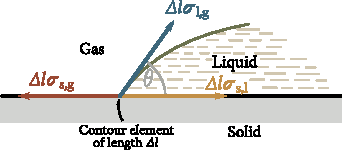
\includegraphics[scale=1]{figures/ch_14/fig_14_7.pdf}
			\caption[]{}
			\label{fig:14_7}
		\end{center}
	\end{minipage}
	\vspace{-0.4cm}
\end{figure}

%If three substances, namely, a solid, a liquid, and a gas, are in direct contact with one another (\fig{14_7}), then the entire system takes on a configuration corresponding to the minimum of the total energy (surface, in the field of forces of gravity, etc.) In particular, the contour along which the three substances are in contact is arranged on the surface of the solid so that the sum of the projections of all the surface tension forces applied to each contour element onto the direction in which the contour element can move (\ie, onto a direction tangent to the surface of the solid) equals zero. It can be seen from \fig{14_7} that the condition of equilibrium of a contour element of length $\Delta l$ is

Nếu có ba chất cùng giới hạn lẫn nhau một lúc: chất rắn, chất lỏng và chất khí (\fig{14_7}), thì cả hệ sẽ có một cấu hình tương ứng với cực tiểu của năng lượng tổng cộng (năng lượng mặt ngoài, năng lượng trong trọng trường, v.v...). Đặc biệt, đường viền nầm tại biên chung của cả ba chất sẽ nằm trên mặt của chất rắn sao cho tổng hình chiếu của tất cả các lực căng mặt ngoài tác dụng lên mỗi yếu tố của đường viền trên phương mà dọc theo đó yếu tố đường viền có thể di chuyển được (tức là phương tiếp tuyến với mặt vật rắn) phải bằng không. Từ \fig{14_7} suy ra là điều kiện cân bằng của yếu tố đường viền có chiều dài $\Delta l$ sẽ được viết như sau:

\begin{equation}\label{eq:14_5}
	\Delta l \ab{\sigma}{s,g} = \Delta l \ab{\sigma}{s,l} + \Delta l \ab{\sigma}{l,g}\cos\theta
\end{equation}

\noindent
%where $\ab{\sigma}{s,g}, \ab{\sigma}{s,l}$ and $\ab{\sigma}{l,g}$ are the surface tensions at the solid-gas, solid-liquid, and liquid-gas interfaces.

Trong đó $\ab{\sigma}{s,g}, \ab{\sigma}{s,l}$ và $\ab{\sigma}{l,g}$ là suất căng mặt ngoài tại các  biên: chất rắn -- khí, chất rắn -- chất lỏng và chất lỏng -- khí.

%The angle $\theta$ measured inside the liquid between tangents to the surface of the solid and the surface of the liquid is called the \textbf{contact angle}. In accordance with \eqn{14_5}, we have

Góc $\theta$ giữa các tiếp tuyến với mặt chất rắn và mặt chất lỏng được tính phía bên trong chất lỏng được gọi là \textbf{góc bờ}. Theo \eqn{14_5}, ta có

\begin{equation}\label{eq:14_6}
	\cos\theta = \frac{\ab{\sigma}{s,g} - \ab{\sigma}{s,l}}{\ab{\sigma}{l,g}}.
\end{equation}

\noindent

%The contact angle is determined by \eqn{14_6} only provided that

Góc bờ được xác định bằng \eqn{14_6} chỉ tính được với điều kiện là:

\begin{equation}\label{eq:14_7}
	\frac{|\ab{\sigma}{s,g} - \ab{\sigma}{s,l}|}{\ab{\sigma}{l,g}} \leqslant 1.
\end{equation}

\noindent

%If this condition is not observed, \ie, $|\ab{\sigma}{s,g} - \ab{\sigma}{s,l}|>\ab{\sigma}{l,g}$, then equilibrium cannot set in at any value of $\theta$. This occurs in two cases.

Nếu điều kiện đó không được thoả mãn, tức là $|\ab{\sigma}{s,g} - \ab{\sigma}{s,l}|>\ab{\sigma}{l,g}$ thì không có giá trị nào của góc $\theta$ có thể đạt tới trạng thái cân bằng. Điều đó xảy ra trong hai trường hợp.

\begin{enumerate}[1.]
	%\item $\ab{\sigma}{s,g}>\ab{\sigma}{s,l}+\ab{\sigma}{l,g}$. No matter how small the angle $\theta$ is, the	force $\ab{\sigma}{s,g}$ overbalances the other two (\fig{14_8}a). In this case, the liquid flows unlimitedly over the surface of the solid---\textbf{complete wetting} takes place. The replacement of a solid-gas interface with two interfaces-solid-liquid and liquid-gas ones---is advantageous from the energy viewpoint. The contact angle is zero in complete wetting.

    \item $\ab{\sigma}{s,g}>\ab{\sigma}{s,l}+\ab{\sigma}{l,g}$. Góc $\theta$ nhỏ tuỳ ý, lực $\ab{\sigma}{s,g}$ cũng lớn hơn hai lực kia (\fig{14_8}a). Trong trường hợp này, chất lỏng chảy rộng ra theo mặt vật rắn nghĩa là ta có \textbf{sự làm ướt hoàn toàn}. Việc thay mặt ngoài chất rắn -- khí bằng hay mặt ngoài chất rắn -- chất lỏng và chất lỏng -- khí thì có lợi hơn về phương diện năng lượng. Trong sự làm ướt hoàn toàn góc bờ là bằng không.
	
	%\item $\ab{\sigma}{s,l}>\ab{\sigma}{s,g}+\ab{\sigma}{l,g}$. No matter how close to $\pi$ the angle $\theta$ is, the force $\ab{\sigma}{s,l}$ overbalances the other two (\fig{14_8}b). In this case, the liquid-solid interface contracts into a point, and the liquid separates from the surface of the solid---\textbf{complete non-wetting} takes place. The replacement of a solid-liquid interface with two interfaces---solid-gas and liquid-gas ones---is advantageous from the energy viewpoint. In complete non-wetting, the contact angle is $\pi$.

    \item $\ab{\sigma}{s,l}>\ab{\sigma}{s,g}+\ab{\sigma}{l,g}$. $\theta$ gần với $\pi$ tuỳ ý, lực $\ab{\sigma}{s,l}$ cũng lớn hơn hai lực kia (\fig{14_8}b). Trong trường hợp này mặt ngăn cách giữa chất lỏng và chất rắn co lại thành một điểm; chất lỏng được tách ra khỏi mặt chất rắn nghĩa là ta có hiện tượng \textbf{hoàn toàn không làm ướt}. Việc thay thế mặt ngoài chất rắn -- chất lỏng bằng hai mặt ngoài chất rắn -- khí và chất lỏng -- khí có lợi hơn về mặt năng lượng. Trong sự hoàn toàn không làm ướt góc bờ là bằng $\pi$.
    
\end{enumerate}

\begin{figure}[!htb]
	\begin{center}
		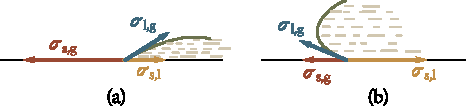
\includegraphics[scale=1.1]{figures/ch_14/fig_14_8.pdf}
		\caption[]{}
		\label{fig:14_8}
	\end{center}
	\vspace{-0.75cm}
\end{figure}

%When condition~\eqref{eq:14_7} is observed, the contact angle may be acute or obtuse depending on the relation between $\ab{\sigma}{s,g}$ and $\ab{\sigma}{s,l}$. If $\ab{\sigma}{s,g}$ is greater than $\ab{\sigma}{s,l}$ then $\cos\theta>0$ and the angle $\theta$ is acute (\fig{14_9}a). In this case, partial wetting occurs. If $\ab{\sigma}{s,g}$ is smaller than $\ab{\sigma}{s,l}$ then $\cos\theta<0$ and the angle $\theta$ is obtuse (\fig{14_9}b). In this case, partial non-wetting occurs.

Khi điều kiện~\eqref{eq:14_7} được thoả mãn, góc bờ có thể là góc nhọn hoặc góc tù phụ thuộc vào hệ thức giữa $\ab{\sigma}{s,g}$ và $\ab{\sigma}{s,l}$. Nếu $\ab{\sigma}{s,g}$ lớn hơn $\ab{\sigma}{s,l}$ thì $\cos\theta>0$ và góc $\theta$ là góc nhọn (\fig{14_9}a). Trong trường hợp này có sự làm ướt một phần. Nếu $\ab{\sigma}{s,g}$ nhỏ hơn $\ab{\sigma}{s,l}$ thì $\cos\theta<0$ và góc $\theta$ là góc tù (\fig{14_9}b). Trong trường hợp này, ta có sự không làm ướt một phần.

%Non-wetting may result in interesting phenomena. It is general knowledge that a needle or safety razor blade coated with grease can float on the surface of water. It is very simple to explain this, at first sight, curious phenomenon on the basis of energy considerations. The greased surface of steel is not wetted by water; the steel-water interface has a much greater energy than the steel-air or air-water ones. The complete submersion of a needle into water is attended by an increase in the surface energy from $S\ab{\sigma}{s,g}$ (steel-air) to the value $S\ab{\sigma}{s,l}$ (steel-water), where $S$ is the surface area of the needle. The change in the surface energy upon submersion is described by the curve $\ab{E}{sur}$ shown in \fig{14_10}. The symbol $h$ stands for the height of the needle above the bottom of the vessel, $h_0$ is the height of the surface of the liquid above the bottom of the vessel. The dependence of the potential energy of the needle in the field of the Earth's gravitation $\ab{E}{gr}$ on $h$ has the form of a straight line passing through the origin of coordinates. The total energy $\ab{E}{tot}=\ab{E}{sur}+\ab{E}{gr}$ has a minimum when $h=h_0$. This is exactly what permits the needle to float on the surface of the water. If we press on the needle and submerge it to a depth such that the total energy passes through its maximum and begins to decrease, then the needle will submerge further by itself and sink.

Sự không làm ướt có thể dẫn đến những hiện tượng rất lý thú. Ta biết rằng khi bôi mỡ vào một cái kim hoặc lưỡi dao cạo thì có thể thả chúng nổi trên mặt nước. Hiện tượng này hoạt nhìn có vẻ kỳ lạ. Ta có thể giải thích hiện tượng đó một cách đơn giản nhất, xuất phát từ việc nghiên cứu năng lượng. Bề mặt của thép được bôi mỡ không bị nước làm ướt; mặt tiếp xúc thép -- nước có năng lượng lớn hơn nhiều so với mặt thép -- không khí hoặc không khí -- nước. Việc nhúng hoàn toàn chiếc kim vào nước kèm theo sự tăng năng lượng mặt ngoài từ giá trị $S\ab{\sigma}{s,g}$ (thép -- không khí) đến giá trị $S\ab{\sigma}{s,l}$ (thép -- nước) trong đó $S$ là mặt ngoài của chiếc kim. Sự thay đổi năng lượng mặt ngoài khi nhúng kim vào nước được biểu diễn bằng đường cong $\ab{E}{sur}$ trên \fig{14_10}. Chữ $h$ biểu diễn độ cao của chiếc kim trên đáy bình; $h_0$ là chiều cao của bề mặt chất lỏng trên mực đáy bình. Sự phụ thuộc của thế năng của chiếc kim trong trọng trường $\ab{E}{gr}$ vào $h$ có dạng một đường thẳng đi qua gốc toạ độ. Năng lượng toàn phần $\ab{E}{tot}=\ab{E}{sur}+\ab{E}{gr}$; nó có cực tiểu khi $h=h_0$; điều đó cho phép chiếc kim nổi trên mặt nước. Nếu ta ấn chiếc kim cho nó chìm xuống một độ sâu, sao cho năng lượng toàn phần đi qua cực đại và tiếp tục giảm thì chiếc kim sẽ tiếp tục chìm sâu và chìm nghỉm.

\begin{figure}[!htb]
	\begin{minipage}[t]{0.5\linewidth}
		\begin{center}
			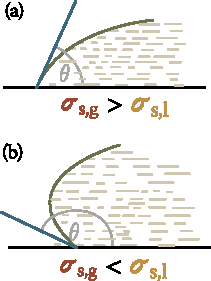
\includegraphics[scale=0.95]{figures/ch_14/fig_14_9.pdf}
			\caption[]{}
			\label{fig:14_9}
		\end{center}
	\end{minipage}
	\hspace{-0.05cm}
	\begin{minipage}[t]{0.5\linewidth}
		\begin{center}
			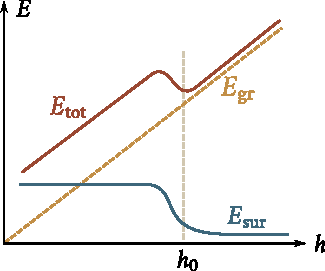
\includegraphics[scale=0.95]{figures/ch_14/fig_14_10.pdf}
			\caption[]{}
			\label{fig:14_10}
		\end{center}
	\end{minipage}
	\vspace{-0.3cm}
\end{figure}

\begin{figure}[t]
	\begin{center}
		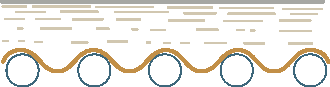
\includegraphics[scale=0.95]{figures/ch_14/fig_14_11.pdf}
		\caption[]{}
		\label{fig:14_11}
	\end{center}
	\vspace{-0.9cm}
\end{figure}

%The possibility of ``carrying water in a sieve'' is explained in a similar way. If water does not wet a sieve (this can be achieved by coating the wires forming the sieve with paraffin) and the layer of water is not very thick, then a slight displacement of the water level downward (\fig{14_11}) will be attended by an increase in the surface energy exceeding in magnitude the decrease in the energy in the field of gravitational forces. Hence, the water will be retained in the sieve and will not spill out.

Ta có thể giải thích một cách tương tự khả năng ''chứa nước trên một tấm lưới''. Nếu nước không làm ướt tấm lưới (ta có thể thực hiện được điều này bằng cách phủ paraffin vào sợi đan tấm lưới) và lớp nước không quá dày thì một sự dịch chuyển của mực chất lỏng xuống dưới một chút (\fig{14_11}) sẽ kèm theo sự tăng của năng lượng mặt ngoài; độ tăng này lớn hơn cả độ giảm của năng lượng trọng trường. Vì vậy nước sẽ được giữ ở trên tấm lưới, không rỏ xuống.

%\section{Capillary Phenomena}\label{sec:14_5}

\section{Các hiện tượng mao dẫn}\label{sec:14_5}

%The existence of the contact angle leads to curvature of the surface of a liquid near the walls of the vessel containing it. In a narrow tube (capillary\footnote{The Latin \textit{capillus} means hair. A capillary is a ``tube as thin as a hair''.}) or in a narrow gap between two walls, the entire surface is curved. If the liquid wets the walls, the surface is concave, and if it does not wet them, the surface is convex (\fig{14_12}). Such curved surfaces of a liquid are called meniscuses.

Sự tồn tại của góc bờ làm cho mặt chất lỏng ở gần thành bình bị uốn cong lên. Trong ống hẹp (ống mao dẫn\footnote{Tiếng Latin \textit{capillus} có nghĩa là tóc. Ống mao dẫn là ống ''mảnh như sợi tóc''.}) hoặc trong khe hẹp nằm giữa hai thành bình thì toàn bộ mặt chất lỏng sẽ bị uốn cong. Nếu chất lỏng làm ướt thành bình, mặt ngoài sẽ có dạng mặt lõm; nếu nó không làm ướt thành bình thì mặt ngoài sẽ có dạng mặt lồi (\fig{14_12}). Những mặt chất lỏng uốn cong loại này gọi là các \textbf{mặt khum}.

%If one end of a capillary is immersed in a liquid poured into a broad vessel, then the pressure under the curved surface in the capillary will differ from that under the flat surface in the broad vessel by the amount $\Delta p$ determined by \eqn{14_4}. As a result, the level of the liquid in the capillary will be higher than in the vessel if the liquid wets it, and lower if the liquid does not wet it.

Nếu ta nhúng một đầu ống mao dẫn vào một chất lỏng chứa trong một bình rộng thì áp suất dưới mặt chất lỏng uốn cong ở trong ống mao dẫn sẽ khác với áp suất dưới mặt phẳng ngoài ở trong bình rộng một lượng là $\Delta p$ xác định bởi \eqn{14_4}. Kết quả là khi chất lỏng làm ướt thành ống mao dẫn, mực chất lỏng ở trong ống sẽ cao hơn mực chất lỏng ở trong bình; khi chất lỏng không làm ướt thành ống thì mực chất lỏng sẽ thấp hơn.

%The change in the height of the liquid level in narrow tubes or gaps has been named \textbf{capillarity}. In the broad meaning of the term, capillary phenomena are understood to include all the phenomena due to the existence of surface tension. In particular, the pressure expressed by \eqn{14_4} and due to surface tension is called, as we have already indicated, capillary pressure. 

Sự thay đổi độ cao của mực chất lỏng trong các ống hẹp hay trong các khe hẹp gọi là \textbf{tính mao dẫn}. Theo nghĩa rộng, ta hiểu mao dẫn là tất cả các hiện tượng gây ra do sự tồn tại của sức căng mặt ngoài. Đặc biệt, áp suất \eqn{14_4} gây ra do sức căng mặt ngoài, như ta đã chỉ ra, gọi là áp suất mao dẫn.

%A difference $h$ sets in between the level of a liquid in a capillary and in a broad vessel such that the hydrostatic pressure $\rho gh$ is balanced by the capillary pressure $\Delta p$:

Giữa chất lỏng ở trong ống mao dẫn và ở trong bình rộng hình thành một sự chênh lệch về độ cao $h$, sao cho áp suất thuỷ tĩnh $\rho gh$ cân bằng với áp suất mao dẫn $\Delta p$:

\begin{equation}\label{eq:14_8}
	\rho gh = \frac{2\sigma}{R}.
\end{equation}

\noindent

%In this equation, $\sigma$ is the surface tension on the liquid-gas interface, and $R$ is the radius of curvature of the meniscus. The latter can be expressed through the contact angle $\theta$ and the radius of the capillary $r$. Indeed, examination of \fig{14_12} shows that $R=r/\cos\theta$. Using this value in \eqn{14_8} and solving the equation obtained relative to $h$, we arrive at the equation

Trong công thức này, $\sigma$ là sức căng mặt ngoài trên biên của chất lỏng -- khí, $R$ là bán kính cong của mặt khum. Ta có thể biểu diễn bán kính cong $R$ của mặt khum theo góc bờ $\theta$ và bán kính $r$ của ống mao dẫn. Thực vậy, từ \fig{14_12}, rõ ràng là $R=r/\cos\theta$. Thế giá trị đó vào \eqn{14_8} và giải phương trình thu được theo $h$, ta được công thức

\begin{equation}\label{eq:14_9}
	h = \frac{2\sigma\cos\theta}{\rho gr}.
\end{equation}

%In accordance with the fact that a wetting liquid rises in a capillary, while a non-wetting liquid lowers in it, \eqn{14_9} gives a positive $h$ for $\theta<\pi/2$ (because $\cos\theta>0$), and a negative $h$ for $\theta>\pi/2$ (because $\cos\theta<0$).

Do ở chỗ chất lỏng làm ướt thành ống sẽ dâng lên trong ống, còn chất lỏng không làm ướt thành ống sẽ tụt thấp xuống, nên trong trường hợp $\theta<\pi/2$ ($\cos\theta>0$), \eqn{14_9} sẽ cho các trị số $h$ dương, còn trong trường hợp $\theta>\pi/2$ ($\cos\theta<0$) sẽ cho các trị số $h$ âm.

%In deriving \eqn{14_9}, we assumed that the meniscus has a spherical shape. The equation for $h$ can also be obtained on the basis of energy considerations, and there is no need to make a special assumption on the shape of the meniscus. The equilibrium position of the meniscus will correspond to a minimum energy $E$ of the liquid-capillary system. This energy consists of the surface energy on the liquid wall, liquid-gas, and wall-gas interfaces, and also of the potential energy of the liquid in the field of the Earth's gravitation.

Khi đưa ra \eqn{14_9} ta đã giả thiết rằng hình dạng của mặt khum là mặt cầu. Ta cũng có thể thu được công thức tính $h$ dựa trên sự nghiên cứu năng lượng, đồng thời ta không cần phải đưa ra một giả thiết đặc biệt gì về hình dạng của mặt khum. Vị trí cân bằng của mặt khum sẽ ứng với cực tiểu của năng lượng $E$ của hệ chất lỏng -- ống mao dẫn. Năng lượng này là tổng của năng lượng mặt ngoài trên các biên chất lỏng -- thành ống, chất lỏng -- khí và thành ống -- khí, và cả thế năng của chất lỏng trong trọng trường.

\begin{figure}[!htb]
	\begin{minipage}[t]{0.5\linewidth}
		\begin{center}
			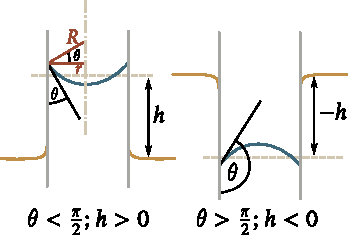
\includegraphics[scale=0.95]{figures/ch_14/fig_14_12.pdf}
			\caption[]{}
			\label{fig:14_12}
		\end{center}
	\end{minipage}
	\hspace{-0.05cm}
	\begin{minipage}[t]{0.5\linewidth}
		\begin{center}
			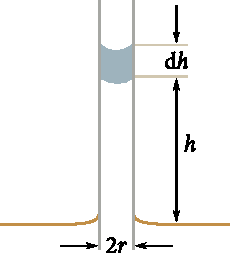
\includegraphics[scale=0.95]{figures/ch_14/fig_14_13.pdf}
			\caption[]{}
			\label{fig:14_13}
		\end{center}
	\end{minipage}
	\vspace{-0.4cm}
\end{figure}

%Let us find the increment of the energy dE corresponding to an increment of the height $\deriv{h}$ to which a liquid rises in a capillary. When the height grows to $\deriv{h}$, the surface area of contact of the liquid with the wall of the capillary increases by $2\pi r\,\deriv{h}$, owing to which the energy receives an increment of $2\pi r\ab{\sigma}{s,l}\,\deriv{h}$. Simultaneously, the surface area of contact between the wall and the gas diminishes, which is attended by an increment of the energy of $-2\pi r\ab{\sigma}{s,g}\,\deriv{h}$. The potential energy in the field of the Earth's gravitation acquires an increment equal to the force of gravity acting on the shaded volume of the liquid (\fig{14_13}) multiplied by $h$, \ie, equal to $g\rho\pi r^2h\,\deriv{h}$. We may disregard the change in the level of the liquid in the broad vessel. Thus,

Ta hãy tính độ tăng của năng lượng $\deriv{E}$ ứng với độ tăng của độ cao cột chất lỏng trong ống mao dẫn một lượng $\deriv{h}$. Khi độ cao tăng lên một lượng là $\deriv{h}$ thì bề mặt tiếp xúc của chất lỏng với thành ống mao dẫn sẽ tăng lên một lượng là $2\pi r\,\deriv{h}$, do đó năng lượng sẽ tăng một lượng là $2\pi r\ab{\sigma}{s,l}\,\deriv{h}$. Đồng thời bề mặt tiếp xúc giữa thành ống và chất khí giảm đi, điều đó kèm theo số gia của năng lượng bằng $-2\pi r\ab{\sigma}{s,g}\,\deriv{h}$. Thế năng trong trọng trường tăng một lượng bằng tích của trọng lực tác dụng lên phần thể tích chất lỏng có gạch chéo (\fig{14_13}) với $h$, tức là bằng $g\rho\pi r^2h\,\deriv{h}$. Ta bỏ qua sự thay đổi của mực chất lỏng trong bình rộng. Vì vậy

\begin{equation*}
	\deriv{E} = 2\pi r\parenthesis{\ab{\sigma}{s,l} - \ab{\sigma}{s,g}}\,\deriv{h} + g\rho\pi r^2h\,\deriv{h}.
\end{equation*}

\noindent

%Hence,
Từ đó suy ra rằng

\begin{equation*}
	\diff{E}{h} = 2\pi r\parenthesis{\ab{\sigma}{s,l} - \ab{\sigma}{s,g}} + g\rho\pi r^2h.
\end{equation*}

\noindent

%Equating this derivative to zero, we obtain the condition of equilibrium, from which it follows that
Cho đạo hàm đó bằng không, ta thu được điều kiện cân bằng; từ đó suy ra

\begin{equation}\label{eq:14_10}
	h = \frac{2\parenthesis{\ab{\sigma}{s,l} - \ab{\sigma}{s,g}}}{g\rho r}.
\end{equation}

\noindent

%According to \eqn{14_6}, $\ab{\sigma}{s,l} - \ab{\sigma}{s,g} = \ab{\sigma}{l,g}\cos\theta$. Making this substitution in \eqn{14_10} and using simply $\sigma$ instead of $\ab{\sigma}{l,g}$ we get \eqn{14_9}.

Theo \eqn{14_6}, $\ab{\sigma}{s,l} - \ab{\sigma}{s,g} = \ab{\sigma}{l,g}\cos\theta$. Thay thế giá trị đó vào \eqn{14_10} và ký hiệu $\ab{\sigma}{l,g}$ đơn giản là $\sigma$, ta thu được \eqn{14_9}.